\documentclass{beamer}
\usepackage{graphicx}
\usetheme{metropolis}           % Use metropolis theme
\title{Multi-Document Summarization: Evaluation, Extraction, and Abstraction}
\date{\today}
\author{Chris Kedzie}
\institute{Dept. of Computer Science, Columbia University}
\begin{document}
  \maketitle
  \section{Evaluation}


\begin{frame}{Evaluating Summarization}
\cite{lin2004rouge} -- ROUGE is the most prevalent automatic measurement tool
 in use for summarization task.
\begin{itemize}
\item recall focused, measures average overlap of system/human summary ngrams
\item many shades: ngram sizes 1 - 9, skip-grams, longest common subsequence 
\item Strong correlation with single doc human coverage scores
\item Reasonable correlation with multi-doc converage scores 
    (largest sample size only 59)
\end{itemize}
\end{frame}

\begin{frame}{Evaluating Summarization}
Criticisms of ROUGE:
\begin{itemize}
\item insensitive to lexical variation
\item uniformly rewards sequence matches, e.g.``of the'' probably not indicative of anything
\item insensitive to linguistic quality, e.g. coherence or disource
\item correlation for MDS is only strong at the 200 and 400 word length
\end{itemize}
\end{frame}

\begin{frame}{Evaluating Summarization}

\cite{hovy2006automated} -- Basic Elements (BE) uses phrase head/modifier words
 as unit of analysis

\begin{itemize}
\item High correlation with responsivenss scores and ROUGE
\item Unclear if BE tells us anything ROUGE doesn't
\item more computationally expensive -- requires parser
\item \cite{owczarzak2009evaluation} found BE to be more unstable under different number of model summaries
\end{itemize}
\end{frame}

\begin{frame}{Evaluating Summarization}
\cite{teufel2004evaluating} develop annotation guidelines for factoid 
definition and annotation, summaries ranked by \# of factoids they contain
\begin{itemize}
\item high agreement on annotation
\item moderate agreement on definition
\item takes 20-30 reference summaries for ranking to stabilize!
\item poor correlation to DUC information overlap?!
\end{itemize} 
\end{frame}

\begin{frame}{Evaluating Summarization}
\cite{nenkova2007pyramid} -- Pyramid: annotation scheme for extracting 
    summary content units (SCUs) from model summaries \\
    system summaries score by importance weighted sum of SCUs they contain
\begin{itemize}
\item score differences stabilize with 4-5 model summaries (compared to 
    20-30 in \cite{teufel2004evaluating})
\item moderate interannotator aggreement on peer annotation
\item strong interannotator score correlation 
\end{itemize} 

\end{frame}

\begin{frame}{Explaining Variation in Evaluation Metrics}

\cite{nenkova2005automatic} -- ANOVA on official DUC coverage scores
\begin{itemize}
\item controlled for system and input (and length in MDS)
\item (generic MDS) differences between systems and baseline are not 
    significant for word lengths 50 and 100  
\item  (generic SDS) no system outperforms baseline; 8/10 humans outperform 
    baseline 
\end{itemize}

\end{frame}

\begin{frame}{Explaining Variation in Evaluation Metrics}
\cite{owczarzak2009evaluation} -- examines stability of system ranking with
    automatic evaluation against TAC Responsiveness Scores  
\begin{itemize}
\item examined Pyramid, ROUGE-2, ROUGE-SU4, and Basic Elements
\item correlation to manual metrics stabilizes after 2 models
\item Contrary to \cite{teufel2004evaluating}, argues for more system inputs 
    with fewer human models 
\end{itemize}
\end{frame}

\begin{frame}{Evaluation without Human Models}
\cite{louis2009automatically} -- examines correlation between input/summary 
    features and TAC08 responsiveness and pyramid scores.
\begin{itemize}
\item (per system) Jensen-Shannon Divergence highly correlated with metrics \\
 $\displaystyle JS(S||I) = \frac{1}{2}\Big(KL(S||I) + KL(I||S) \Big)$
\item (per input) correlations vary wildly per input \\
  JS max $ =-.714, $ min $ =-.271$
\item (query-focused) high correlation between summary/inputs w/o using query
\item (update) using background documents results in worse correlation
\end{itemize}
\end{frame}


\begin{frame}{Evaluating Update Summaries}
\cite{conroy2011nouveau} -- there is a gap between automatic metrics of human 
 update summaries and machine generated summaries
\begin{figure}
\centering
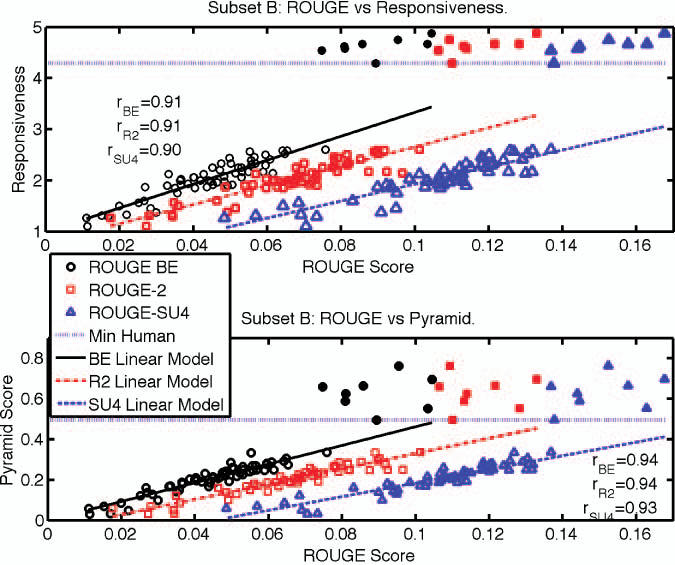
\includegraphics[width=\linewidth,height=.7\textheight,keepaspectratio]{metric_gap_rouge.jpg}
\end{figure}
\end{frame}

\begin{frame}{Evaluating Update Summaries}
\cite{conroy2011nouveau} -- there is a gap between automatic metrics of human 
 update summaries and machine generated summaries
\begin{itemize}
\item $NouveauRouge = \alpha_{AB} Rouge(A,B) + \alpha_{BB} Rouge(B,B) + \alpha_0$
\item $Rouge(A,B) \triangleq$ ROUGE score of system update summary to 
         model original summary
\item $Rouge(B,B) \triangleq$ ROUGE score of system update summary to 
         model update summary
\item in fitted model: 
\begin{itemize}
\item $\alpha_{A,B} < 0$ 
\item $\alpha_{B,B} > 0$ 
\end{itemize}
\end{itemize}

\end{frame}

\section{Extraction}

\begin{frame}{Heuristics}
\cite{nenkova2005impact} -- isolate the effects of frequency for extraction
  
\begin{itemize}
\item very competetive ROUGE performance
\item greedy algorithm for computing summaries 
 \item performance possibly due to reweighting, 
\begin{itemize}
\item unreweighted summaries have 
    much lower ROUGE
\item unreweighted algo. is approx. of document likelihood objective in \cite{louis2009automatically}, which poorly correlates with human judgements
\end{itemize}
\end{itemize}

\end{frame}

\begin{frame}{Heuristics}
\cite{nenkova2005impact} -- examine weighting pyramid annotations (potentially remove need for model 
    summary annotation)
\begin{itemize}
\item strong but imperfect correlation
\item frequency does not fully explain content selection
\begin{figure}
\centering
\begin{tabular}{l| l| l| l}
         & Top 5              & Top 8              & Top 12  \\
\hline
human    & \alert<2>{94.66\%} & \alert<3>{91.25\%} & \alert<4>{85.25\%} \\
\hline
machine  & 84.00\%            & 77.87\%            & 66.08\% \\
\hline
SumBasic & \alert<2>{96.00\%} & \alert<3>{95.00\%} & \alert<4>{90.83\%} \\
\end{tabular}

\end{figure}
\item SumBasic consistently \alert<2->{over-estimates} frequency importance vs human
\end{itemize}
\end{frame}

\begin{frame}{Heuristics}
\cite{lin2000automated} -- automatic method for finding key phrases/terms 
    using likelihood ratios
\begin{itemize}
\item $\mathcal{R} \triangleq$ relevant docs; 
    $\tilde{\mathcal{R}} \triangleq$ irrelevant docs;
    $t \triangleq $ ngram 
\item Hypothesis 1 ($H_1$): $P(\mathcal{R}|t) = P(\tilde{\mathcal{R}}|t)$
\item Hypothesis 2 ($H_2$): $P(\mathcal{R}|t) \gg P(\tilde{\mathcal{R}}|t)$
\item large $L(H_2) \rightarrow $ large  $ -2\log\frac{L(H_1)}{L(H_2)} $
\end{itemize}
\end{frame}


\begin{frame}{Heuristics}
\cite{lin2000automated} -- automatic method for finding key phrases/terms 
    using likelihood ratios
\begin{itemize}
\item ranking sentences by topic signatures outperforms tfidf and lead 
    baselines
\item limited evaluation (only 4 topics)
\item however, \cite{louis2009automatically} find moderate positive 
    correlation between topic signature coverage and human responsiveness 
    scores
\end{itemize}
\end{frame}

\begin{frame}{Random Walks on Sentences}
\cite{erkan2004lexrank} -- Extract sentences via graph-based notion of 
    centrality
\begin{itemize}
\item sentences are \textit{nodes} in a \textit{graph}, 
\item \textit{edges} are weighted by sentence similarity
\item PageRank finds an eigenvector of the adjacency matrix
\item eigenvector elements are interpretable as a ranking of sentence centrality
\end{itemize}
\end{frame}

\begin{frame}{Random Walks on Sentences}
\cite{erkan2004lexrank} -- Extract sentences via graph-based notion of 
    centrality
\begin{itemize}
\item language agnostic
\item generally benefits from reranking to handle redundancy
\end{itemize}
\end{frame}

\begin{frame}{Query Focused Summarization}
\cite{conroy2005classy} -- use query term and topic signature matches as 
    features in an hidden Markov model (HMM).
\begin{itemize}
\item selection with HMM, requires extractive gold summaries
\item reranking step performed with pivoted QR decomposition
\item Named Entity (NE) tagging not helpful, despite HACKY exploitation of 
    ROUGE-1
\item High pyramid scores, despite low ROUGE-1 performance
\end{itemize}
\end{frame}


\begin{frame}{Streaming Summarization}
\cite{guo2013updating} -- define streaming summarization task, exploratory
    system design and evaluation
\begin{itemize}
\item explore sentence selection from first 10 sentences or headline only
\item effects of stationary/non-stationary features
\item non-stationary features introduce importance of buffering policy
\item feature combination for first 10 sentences best overall
\end{itemize}
\end{frame}

\begin{frame}{Streaming Summarization}
\cite{mccreadie2014incremental} -- Streaming summarization systems are noisy
    during periods of downtime; learn to predict rank cutoff to reduce noise
\begin{itemize}
\item this task is hard -- very large gap between oracle and current top 
    performance
\item improved recall measure but precision? Counter-intuitive result? 
\end{itemize}
\end{frame}

\begin{frame}{Summarization in other Domains}
\cite{maskey2005comparing} -- Broadcast news speech summarization
\begin{itemize}
\item Prosodic/Acoustic features complement lexical features
\item Suggests speech summarization without transcription is possible
\end{itemize}
\end{frame}

\begin{frame}{Summarization in other Domains}
\cite{titov2008joint} -- Review/Opinion summarization; Correlate LDA-style 
    topics with ratings values
\begin{itemize}
\item model allows for extraction of sentences for different aspects of review
\item very competitive with a supervised extractive model 
\end{itemize}
 
\end{frame}


\begin{frame}{Summarization in other Domains}
\cite{gillick2009global} -- Meeting summarization; use ILP solver to maximize
    ngram coverage subject to length and speaker constraints
\begin{itemize}
\item were able to obtain oracle ROUGE scores
\item remaining improvement should be found in improving coherence and other
    linguistic qualities 
\end{itemize}
\end{frame}

\begin{frame}{Summarization in other Domains}
\cite{liu2011sxsw} -- Twitter summarization; use ILP solver to maximize
    ngram coverage subject to length and speaker constraints
\begin{itemize}
\item compare multiple input sources: tweets/normalized tweets or linked web
 text, or combination 
\item only tiny variation in ROUGE depending on input
\item Web Text inputs yield higher grammaticality scores
\item Tweet inputs yield higher clarity and focus scores
\end{itemize}
\end{frame}



\bibliographystyle{apalike}
\bibliography{references}


\end{document}

